\documentclass{article}


\usepackage{arxiv}

\usepackage[utf8]{inputenc} % allow utf-8 input
\usepackage[T1]{fontenc}    % use 8-bit T1 fonts
\usepackage{hyperref}       % hyperlinks
\usepackage{url}            % simple URL typesetting
\usepackage{booktabs}       % professional-quality tables
\usepackage{amsfonts}       % blackboard math symbols
\usepackage{xfrac}       % compact symbols for 1/2, etc.
\usepackage{microtype}      % microtypography
\usepackage{array}
\usepackage{graphicx}
\graphicspath{ {./images/} }

\title{A Review of Lossless Data Compression Algorithms}


\author{
	Aditya Meharia\\
	School of Computer Engineering\\
	Kalinga Institute of Industrial Technology\\
	Bhubaneswar, India 751024 \\
	\texttt{adityameharia14@gmail.com} \\
  	%% examples of more authors
	\And
   	Junaid H. Rahim\\
	School of Computer Engineering\\
	Kalinga Institute of Industrial Technology\\
	Bhubaneswar, India 751024 \\
	\texttt{junaidrahim5a@gmail.com} \\	
}

\begin{document}
\maketitle

\begin{abstract}
	

This work aims to provide an introduction to the domain of Data Compression in Information Theory and a comprehensive review of the existing literature in the field of algorithms for Lossless Data Compression. We identify and discuss the potential opportunities, barriers and the future scope of the field. We also review data compression methods used for text, image, video and  audio data.

%\subsection*{Results}
%Mostly about which algo performs best for what kinda field and all that. will write this later when the paper is complete. thats a reference example



\end{abstract}

\keywords{Data Compression \and Algorithms \and Lossless Data Compression \and Information Theory}


\section{Introduction}

A rapid growth in modern communication technology led an explosion in the amount of data we transmit and store. Large files consume significant resources for transmission as well as storage. Due to this exponential increase in the size of the data we transmit, researchers developed algorithms that can be used to compress the data to save storage space as well as transmission time. Data Compression is a process by which we encode the input data into a representation that occupies fewer bits than the original input. This encoded representation is transmitted and decoded back to the original form at the destination. Data compression algorithms are broadly classified into two classes viz \textbf{Lossless Compression} and \textbf{Lossy Compression} algorithms. We will be only covering Lossless Data Compression algorithms in this review article.

\subsection{History of Data Compression}

The field of data compression gained huge significance in the 1970s after the surge in the usage of the internet. The need to reduce transmission time pushed computer scientists to find new ways to compress information. Although, the very earliest form of compression was Morse Code, invented in 1838, in Morse code the letters 'e' and 't' from the english language were given shorter codes as they have a high probability of occurrence.

Later with the advent of mainframe computers, Calude Shanon and Robert Fano invented Shanon-Fano coding in 1949\cite{shannon1948mathematical}, the algorithm assigns shorter codes to symbols with high probability resulting in a shorter way to represent the data. In 1952, David Huffman, one of the students of Robert Fano at MIT studying information theory took the option to write a term paper when given a choice between taking a final exam or writing a paper. Huffman was interested in finding the most efficient way to assign prefix codes to a set of symbols, after months of work Huffman published Huffman Coding in his paper "A Method for the Construction of Minimum-Redundancy Codes"\cite{huffman1952method}, Huffman coding was an improvement over Shanon-Fano coding in terms of efficiency as it assured the assignment of the shortest possible codes to the given symbols. The early implementations of Shanon-Fano coding and Huffman coding were done using hardcoded codes, later in the 1970s, software compression was implemented and Huffman Codes were dynamically generated depending on the input data.

In 1977, Abraham Lempel and Jacob Ziv published\cite{ziv1977universal} their groundbreaking LZ77 algorithm and later the LZ78 algorithm, these algorithms used a dictionary to compress data. The popular UNIX operating system used a compression utility based on LZW which was a slight modification of the LZ78 algorithm. Later the UNIX community adopted the DEFLATE based gzip and Burrows-Wheeler transform based bzip2 formats mostly due to their open source nature\cite{burrows1994block}. It was a beneficial decision in the long run as gzip and bzip2 have consistently given higher compression ratios compared to the LZW format.


In 1989, Phil Katz released the PKZIP format, later in 1993 Katz updated the format and named it PKZIP 2.0, he based it on the DEFLATE algorithm, the .zip format used so extensively in today's day is  based on the PKZIP 2.0 format. ZIP and other DEFLATE based formats were extremely popular till the mid 1990s when new and improved formats began to emerge. In 1993, Eugene Roshal released his WinRAR utility which uses the proprietary RAR format. The RAR format is one of the most used formats to compress data and share it via the internet. In 1999, UNIX adopted the 7-zip or the .7z format, this was the first one capable enough to challenge the dominance of the .zip and .rar formats as .7z was not limited to just one compression algorithm, but could instead choose any of bzip2, LZMA, LAMA2 and PPMd algorithms among others. 




\subsection{Overview of Lossless Data Compression Techniques}

Lossless Compression algorithms are a class of algorithms that can reproduce the original content from the encoded respresentation without any loss of information, the data before compression and after decompression is exactly the same. Lossless compression is used in a variety of fields where it is important that the original and decompressed information be the same. The GNU tool gzip uses lossless algorithms for the ZIP file format.

Lossless compression algorithms usually have a two step procedure. 
\begin{enumerate}
	\item A statistical model of the input data is generated. This usually assigns a probability of occurrence to pieces of input data. For example, if the input data is piece of text, then the model would be the probabilities of occurance of each alphabet
	
	\item A coding system uses this model to map the data in a way that the pieces with high probability of occurrence are assigned a shorter code than those with a low probability of occurance
\end{enumerate}

The probabalistic model is usually generated in two ways, a static way and an adaptive/dynamic way. In the static approach, the data is analysed and the probability model is generated before starting the encoding procedure, this is a modular and simple approach but doesn't perform well for heterogeneous data since the approach forces the use of a single model for the all the data. In the dynamic method, the model is updated while compressing the data. The encoder and decoder start with a trivial model in the initial state, thus performs poorly on initial data, but as the model adapts to the data, the performance improves. Most efficient compression techniques usually employ an adaptive model. There are various ways to achieve losseless compression namely Run Length Encoding (RLE), Lossless predictive coding (LPC), Entropy coding and Arithmetic coding etc.\cite{parekar2014lossless}\cite{yellamma2012performance}

\section{Prefix Codes and Entropy}

A prefix code is a "code" system in which the codes given to each character is not the prefix of the code given to any other character i.e. it follows the prefix property \cite{berstel1985theory}. For example $\{2,42,12\}$ is an example of a prefix system whereas $\{2,42,12,21\}$ is not because '2' is the prefix of '21'.

Prefix codes are also known as prefix-free codes, prefix condition codes and instantaneous codes. They are uniquely decodable codes that is no two codes will have the same value on decoding. Prefix codes can be both fixed length and of variable length. It does not require between words to seperate them. Variable length preifx codes have been used extensibly in Huffman and Shannon coding and are still used in modern compression algorithms along with arithmetic coding.

Entropy denotes the randomness of the data that you are passing as input to the compression algorithm. That means the more random the text i.e. higher entropy is, the lesser you can compress it. It represents an absolute limit on the best possible lossless compression of any communication: treating messages to be encoded as a sequence of independent and identically distributed random variables. Shannon's source coding theorem shows that, the average length of the shortest possible representation to encode the messages in a given alphabet is expressed as follows

Given a random variable $X$, with possible outcomes $x_{i}$, each with probability $P_{X}(x_{i})$, the entropy $H(X)$ of $X$, where $b$ is the base of the logarithm is as follows:

$$H(X) = - \sum_{i=1}^{n} P_X(x_{i}) \log_{b} P_X(x_{i}) = \sum_{i=1}^{n} P_X(x_{i})I_X(x_{i}) = E[I_X] $$


\section {Shanon Coding}

It is named after its creator \textbf{Claude Shanon}, the technique was used to prove Shanon's noiseless coding theorem in his 1948 article "A Mathematical Theory of Communication"\cite{shannon1948mathematical}. Even though being suboptimal, the method was a first of its kind. This method is credited to have given rise to the entire field of Information Theory. Some of the most efficient compression algorithms today are usually an exntension of shanon's method

Shanon Coding is a method to generate prefix codes for a given piece of data. It is done using the occurrence probabilities of the pieces of data. First the probabilities $p_{i}$ are arranged in descending order, then each piece is assigned a code which is the first $l_{i}$ digits of binary representation of the cumulative probability till that piece of data. 


Given that the probability of occurrence is $p_{i}$, the cumulative probability is expressed as 
$$\sum_{k=0}^{i-1} p_{k}$$ where $l_{i} = \left \lceil \log_{2} p_{i} \right \rceil$ 

It is a suboptimal algorithm, it does not give the lowest possible code word length.

The following is an example of assigning prefix codes to compress the string "lossless data compression"


\begin{center}
	\begin{tabular}{ccccccl}
		\toprule
		$i$ & $a_{i}$ &     $p_{i}$ &  $p_{c} = \sum\limits_{k=0}^{i-1} p_{k}$ &    Binary Representation &  $l_{i} = \left \lceil \log_{2} p_{i} \right \rceil$ &  code \\
		\midrule
		0  &        s &  0.24 &          0.00 &  0.00000000... &               2 &    00 \\
		1  &        o &  0.12 &          0.24 &  0.00111101... &               3 &   001 \\
		2  &        e &  0.08 &          0.36 &  0.01011100... &               3 &   010 \\
		3  &   <space>  &  0.08 &          0.44 &  0.01110000... &               3 &   011 \\
		4  &        a &  0.08 &          0.52 &  0.10000101... &               3 &   100 \\
		5  &        l &  0.08 &          0.60 &  0.10011001... &               3 &   100 \\
		6  &        i &  0.04 &          0.68 &  0.10101110... &               4 &  1010 \\
		7  &        d &  0.04 &          0.72 &  0.10111000... &               4 &  1011 \\
		8  &        t &  0.04 &          0.76 &  0.11000010... &               4 &  1100 \\
		9  &        c &  0.04 &          0.80 &  0.11001100... &               4 &  1100 \\
		10 &        m &  0.04 &          0.84 &  0.11010111... &               4 &  1101 \\
		11 &        r &  0.04 &          0.88 &  0.11100001... &               4 &  1110 \\
		12 &        p &  0.04 &          0.92 &  0.11101011... &               4 &  1110 \\
		13 &        n &  0.04 &          0.96 &  0.11110101... &               4 &  1111 \\
		\bottomrule
	\end{tabular}
\end{center}


 
\section {Huffman Coding}
Named after its creator David A. Huffman. Although C.E. Shannon \cite{shannon1948mathematical} and R.M.Fano \cite{fano1949transmission} developed ensemble coding procedures to prove that the average number of binary digits required per message approaches from above the average amount of information per message,it was not optimum. Kraft \cite{kraft1949device} had derived a coding method which gives an average code length as close as possible to the ideal when the ensemble contains a finite number of members. However Huffman was able to derive a definte procedure for this. The output of the Huffman table given us a prefix-variable code table which consists of the source symbol and the encoded symbol. 

Like Shannon coding, Huffman algorithm also tries to minimize the entropy by assisgning shortest codes to the charcters which occur most frequently. The algorithm works by creating a binary tree (using a min heap) which can have either leaf nodes or internal nodes. The leaf node contains the weight and the symbol whereas the internal nodes consists of weight and links to the two child nodes. The bit '0' is used to reprsent the left child of an internal nodes whereas the bit '1' is used to represent the right child.

Steps to build a Huffman Tree:-

\begin{enumerate}
	\item The process begins by traversing the input string and finding all the unique charcters along with their frequencies.
	\item Then create a leaf node for each symbol and their frequencies(weight) and add build a min heap of all the leaf nodes.
	\item Take the two nodes with the minimum weight and create a new  internal node with the weight equal to the sum of the frequencies of the 2 nodes.Make the first extracted child as the left node and the second extracted child as the right node and add it to the min heap.
	\item Repeat the steps until the heap contains only one node.
\end{enumerate}

Letter freqency table

\begin{flushleft}
	\setlength{\extrarowheight}{0.2cm}
	\begin{tabular}{|l|l|l|l|l|l|l|l|l|}
		\hline
		Letter    & Z	 & K & M  & C  & U  & D  & L  & E   \\ \hline
		Frequency & 2 & 7 & 24 & 32 & 37 & 42 & 42 & 120 \\ \hline
	\end{tabular}
\end{flushleft}


Huffman Code\

\begin{flushleft}
	\setlength{\extrarowheight}{0.2cm}
	\begin{tabular}{|l|l|l|l|}
		\hline
		Letter & Freq & Code   & Bits \\ \hline
		E      & 120  & 0      & 1    \\ \hline
		D      & 42   & 101    & 3    \\ \hline
		L      & 42   & 110    & 3    \\ \hline
		U      & 37   & 100    & 3    \\ \hline
		C      & 32   & 1110   & 4    \\ \hline
		M      & 24   & 11111  & 5    \\ \hline
		K      & 7    & 111101 & 6    \\ \hline
		Z      & 2    & 111100 & 6    \\ \hline
	\end{tabular}
\end{flushleft}

\begin{center}
	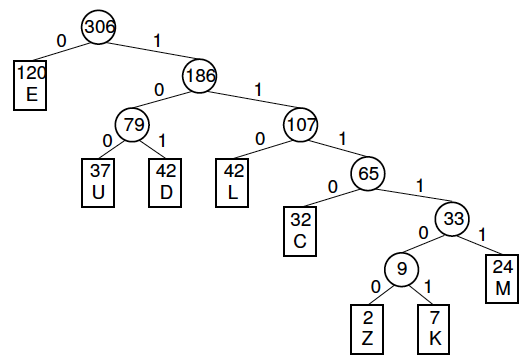
\includegraphics[width=10cm]{huffman_tree}
\end{center}

Decoding the Huffman tree is very simple, traverse the tree node by node as each bit is read from the input stream (reaching a leaf node necessarily terminates the search for that particular byte value). 

For example, decoding an encoded string can be done by looking at the bits in the coded string from left to right until a letter decoded.
10100101 $\Rightarrow$ DEED

\section{Lempel-Ziv(lz) Compression Methods}

\section{Run Length Coding}

\section{Prediction by Partial Matching}

\section{Arithmetic Coding}

\section{Deflate}

\section{Grammar Based Compression}

\section{Current Research Work}

\section{Future Scope}

\section{Conclusion}

\bibliographystyle{unsrt}
\bibliography{main}

\end{document}